\newpage
\section{Reanalysis of Muennighoff et al.\ compute-optimal allocation}
\label{app:muennighoff_reanalysis}

Our scaling law recommends allocating data-constrained compute toward larger models trained for fewer epochs, while \citet{muennighoff2023scaling} recommend the opposite: smaller models trained for more epochs. We trace this disagreement to the fact that \citet{muennighoff2023scaling} fit their Chinchilla base law on \citet{hoffmann2022training}'s scraped C4 isoFLOP points rather than on their own scaling runs. Although both studies use C4, differences in tokenization, preprocessing, and training codebases mean that parameters fit on one set of runs need not transfer to another \citep{li2025misfitting}. Indeed, we show that this baseline fits the \citet{muennighoff2023scaling} single-epoch runs poorly, and that the $\widehat{D}, \widehat{N}$ effective-parameter mechanism primarily compensates for this baseline error. When the Chinchilla base is refit on their own data, the two analyses agree.

All results below use the \citet{muennighoff2023scaling} filtered data split (182 runs) with their outlier-removal criteria, matching their evaluation setup.

\para{The Chinchilla baseline transferred from Hoffmann et al.\ fits poorly.} \autoref{tab:chinchilla_baseline_quality} compares the published Chinchilla parameters against parameters refit on the 29 single-epoch runs from \citet{muennighoff2023scaling}. The published parameters explain only 71.1\% of variance on single-epoch data ($R^2 = 0.711$). Since no repetition is involved, these runs should be well-described by a Chinchilla law. Refitting the Chinchilla parameters to the \citet{muennighoff2023scaling} single-epoch data recovers $R^2 = 0.989$, a near-perfect fit. The 3$\times$ reduction in Huber loss confirms that the original parameters are a poor description of these data. The improvement is not driven by relaxing the $\alpha=\beta$ constraint: a tied refit on the same 29 runs also achieves $R^2 = 0.989$.



\para{The effective-parameter mechanism compensates for baseline error.} \autoref{tab:dprime_nprime_comparison} shows the impact on the $\widehat{D}, \widehat{N}$ scaling law. With the published Chinchilla base, adding the $\widehat{D}, \widehat{N}$ mechanism improves $R^2$ by $+0.346$ (from 0.445 to 0.791)---appearing to provide substantial value. With the refit base, the same mechanism improves $R^2$ by only $+0.070$ (from 0.861 to 0.931). The absolute fit quality improves (Huber 0.0158 $\to$ 0.00720), but the marginal contribution of the $\widehat{D}, \widehat{N}$ mechanism is smaller once the baseline is correct.

The mechanistic explanation is visible in the fitted parameters. Under the published base, the effective-parameter rate constant $R_N^* = 5.31$, meaning effective model size saturates quickly, biasing the optimal allocation toward smaller models. Under the refit base, $R_N^* = 3{,}294$, effectively infinite. The optimizer disables the $\widehat{N}$ mechanism entirely. Without $\widehat{N}$ pulling the allocation toward smaller models, the refit $\widehat{D}, \widehat{N}$ law recommends larger models with fewer epochs which aligns with our independent finding.



\para{The allocation recommendation reverses.} \autoref{fig:muennighoff_reanalysis_allocation} shows the compute-optimal allocation under the published and refit $\widehat{D}, \widehat{N}$ laws at a unique data budget of 25B tokens. The published law (yellow) allocates toward smaller models and more epochs than Chinchilla, consistent with the original recommendation. The refit law (red) reverses direction, allocating toward larger models---consistent with our finding that compute is better spent on model capacity than on data repetition.

\begin{table}[t]
    \centering
    \caption{\textbf{Chinchilla baseline quality on \citet{muennighoff2023scaling} data.} Published parameters (fit on \citet{hoffmann2022training}'s scraped isoFLOP points) vs.\ parameters refit on the 29 single-epoch runs from \citet{muennighoff2023scaling}.}
    \label{tab:chinchilla_baseline_quality}
    \begin{tabular}{lcc}
        \toprule
        Metric & Published & Refit \\
        \midrule
        $R^2$ (all runs) & 0.445 & \textbf{0.861} \\
        $R^2$ (single-epoch) & 0.711 & \textbf{0.989} \\
        $R^2$ (multi-epoch) & 0.306 & \textbf{0.795} \\
        Huber loss & 0.0331 & \textbf{0.0115} \\
        \bottomrule
    \end{tabular}
\end{table}

\begin{table}[t]
    \centering
    \caption{\textbf{Benefit of $\widehat{D}, \widehat{N}$ under published vs.\ refit Chinchilla base.} $\Delta R^2$ is the improvement over the corresponding Chinchilla-only baseline.}
    \label{tab:dprime_nprime_comparison}
    \begin{tabular}{lccccc}
        \toprule
        Condition & $R^2$ (all) & $\Delta R^2$ & $R^2$ (single) & $R^2$ (multi) & Huber Loss $\downarrow$ \\
        \midrule
        Published Chinchilla & 0.445 & --- & 0.711 & 0.306 & 0.0331 \\
        \quad{}$+\;\widehat{D}, \widehat{N}$ (published) & 0.772 & $+0.327$ & 0.763 & 0.777 & 0.0158 \\
        \quad{}$+\;\widehat{D}, \widehat{N}$ (refit) & 0.791 & $+0.346$ & 0.789 & 0.792 & 0.0158 \\
        \midrule
        Refit Chinchilla  & 0.861 & --- & 0.989 & 0.795 & 0.0115 \\
        \quad{}$+\;\widehat{D}, \widehat{N}$ (refit) & 0.931 & $+0.070$ & 0.989 & 0.902 & 0.00720 \\
        \bottomrule
    \end{tabular}
\end{table}

\begin{figure}[t]
    \centering
    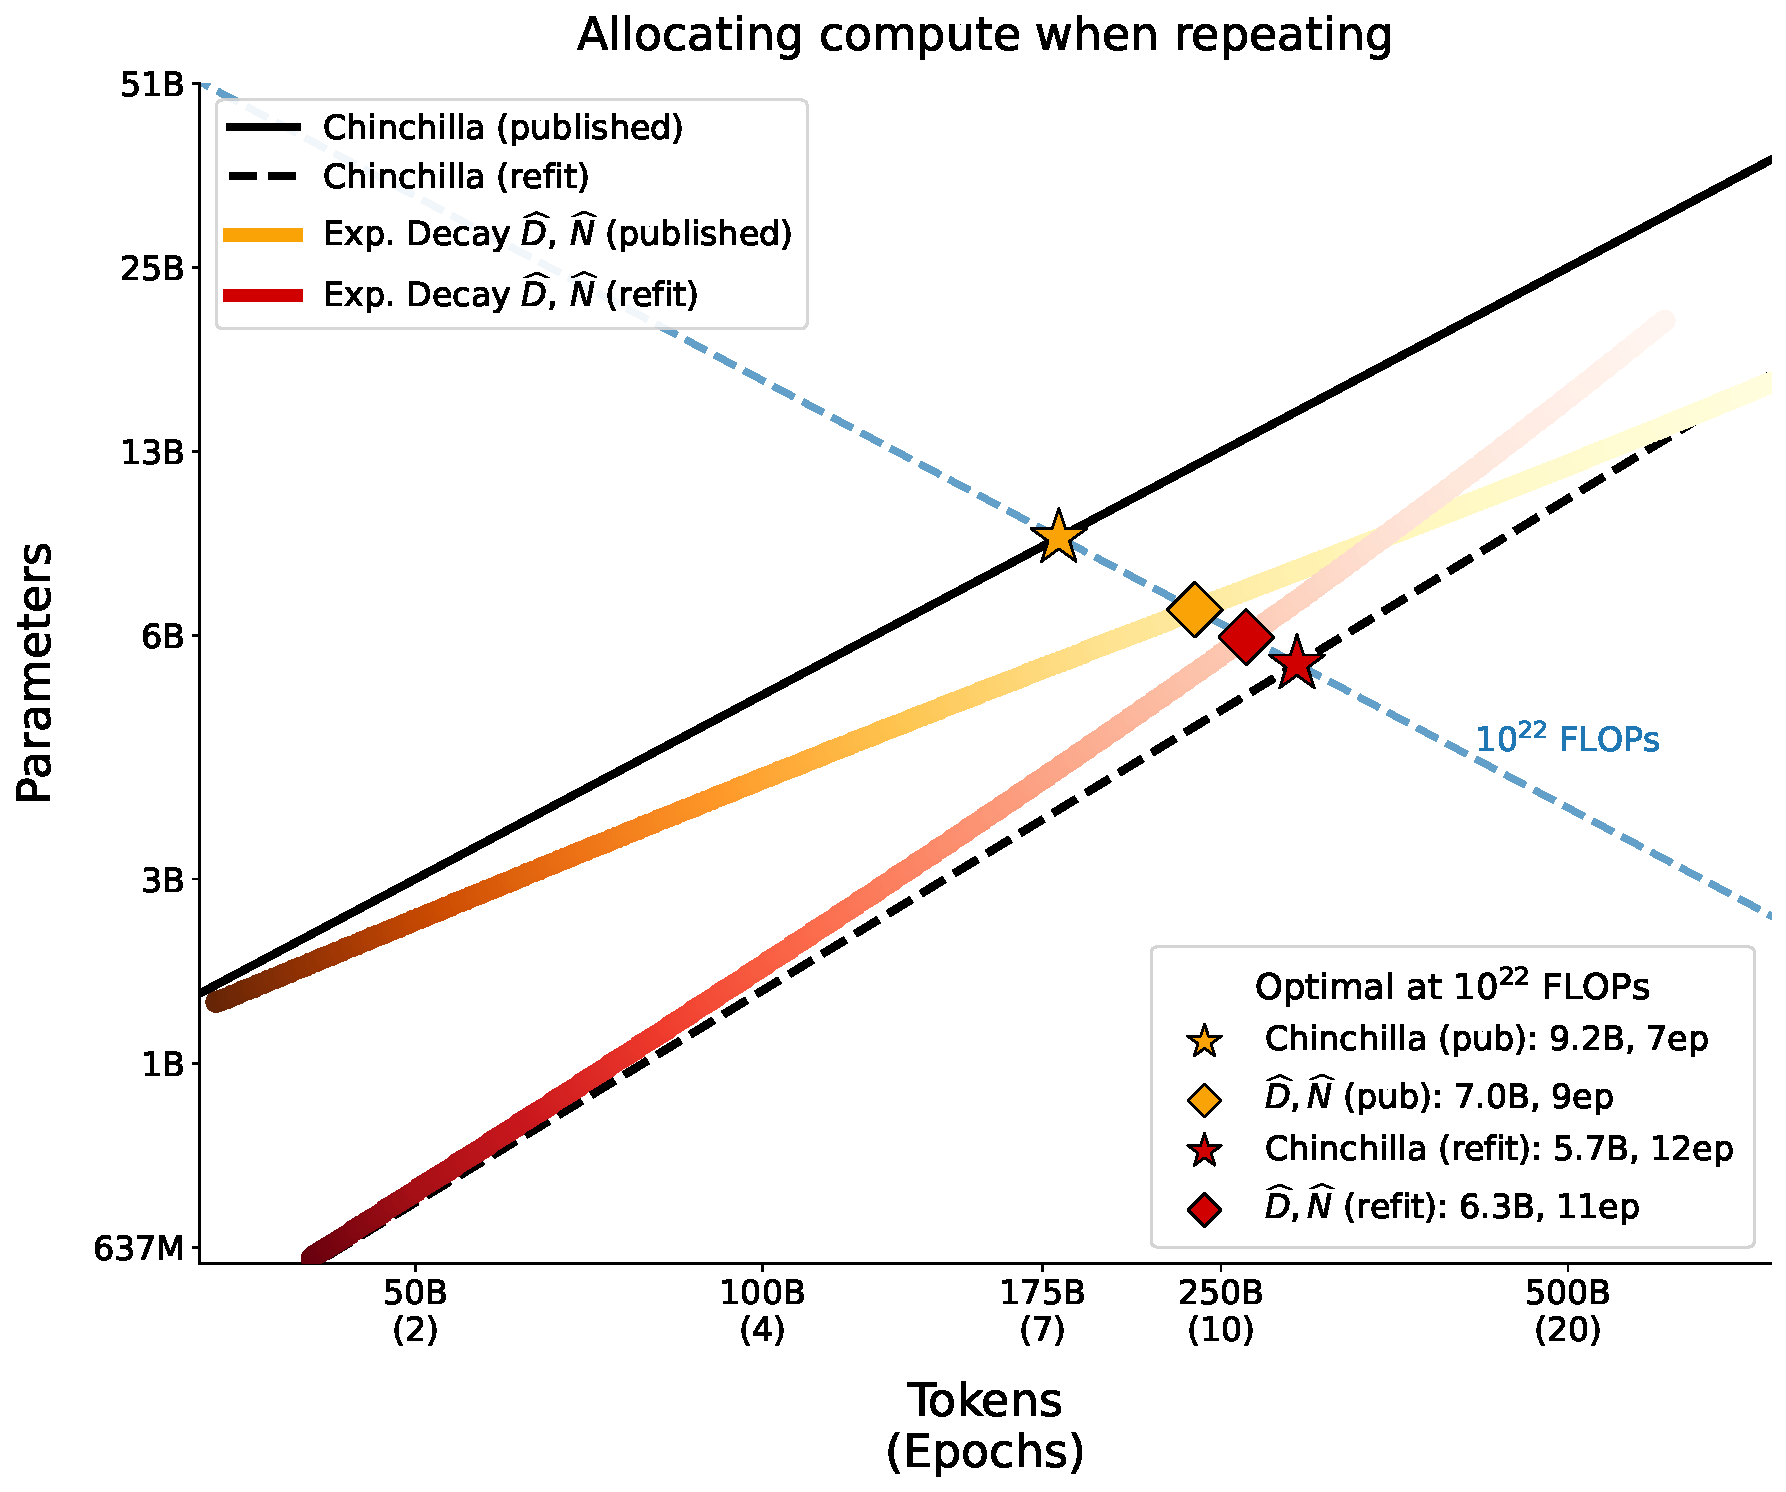
\includegraphics[width=\textwidth]{figures/law_comparison_UD25000M.pdf}
    \caption{\textbf{Compute-optimal allocation reverses under refit Chinchilla base.} Black lines: Chinchilla-optimal (no repetition). Solid lines: $\widehat{D}, \widehat{N}$-optimal. Yellow: published parameters from \citet{muennighoff2023scaling}. Red: refit parameters. The published $\widehat{D}, \widehat{N}$ law allocates toward smaller models and more data than Chinchilla, while the refit law allocates toward larger models, reversing the original recommendation. $U_D = 25$B tokens.}
    \label{fig:muennighoff_reanalysis_allocation}
\end{figure}

In summary, the apparent disagreement between our recommendation and that of \citet{muennighoff2023scaling} reduces to the $\widehat{N}$ mechanism absorbing systematic error from a misspecified Chinchilla baseline. When the baseline is corrected, the $\widehat{N}$ mechanism disables itself and the allocation recommendation aligns with ours. We note that this reanalysis was possible only because \citet{muennighoff2023scaling} made their data and experimental details publicly available.
